\documentclass[a4paper,12pt,oneside,BCOR=0mm,bibliography=totoc,parskip=half]{vwa}
% bibliography=totoc gibt an, dass das Literaturverzeichnis im Inhaltsverzeichnis aufscheinen soll.

% Lädt die Silbentrennungseinstellungen für die neue deutsche Rechtschreibung
% Um weitere Silbentrennungen zu laden, die Sprachen VOR deutsch eintragen (mit Komma getrennt)
% Bei anderssprachigen Arbeiten die jeweilige Sprache als letzte eintragen (mit Komma getrennt)
\usepackage[english,naustrian]{babel}

% Zum Einbinden des Deckblattes als PDF-Datei
\usepackage{pdfpages}

%Zum Erzeugen benutzerdefinierter Bildunterschriften
\usepackage[figurename=Abb.]{caption}
% \usepackage{svg}

% Zum Erzeugen von Bildern
\usepackage{tikz}
\usetikzlibrary{matrix,chains,positioning,decorations.pathreplacing,arrows}

%Paket für benutzerdefinierte Nummerierungen z.B. \begin{enumerate}[(a)]
\usepackage[shortlabels]{enumitem}

% Erzeugt österreichische Anführungszeichen („ und “) und ersetzt " automatisch
% durch die im Kontext richtigen Anführungszeichen.
\usepackage[style=austrian]{csquotes}
\MakeOuterQuote{"}

% \usepackage[style=verbose]{biblatex}

% ---- FORMELSATZ ----------------------------------------------------------------------
% Wird der Formelsatz nicht benötigt, kann alles hier bis zu "allgemeine Information"
% entweder kommentiert (mittels Voranstellen eines % in jeder Zeile) oder gelöscht
% werden.
% Lädt zusätzliche Werkzeuge für den Formelsatz.
\usepackage{mathtools}

% Lädt die American Mathematical Society-Erweiterungen bzgl. Formelsatz:
% amsmath   sind generelle LaTeX-Erweiterungen für den fortgeschrittenen Formelsatz.
% amsfonts  sind moderne Schriften für Formeln incl. skalierbaren Zeichen.
% amssymb   sind erweiterte Zeichensätze für den fortgeschrittenen Formelsatz.
\usepackage{amsmath}
\usepackage{amsfonts}
\usepackage{amssymb}
% \usepackage{pgfplots}
% \pgfplotsset{compat = newest}
% \usepackage{calc}

% Legt den Style von direkten Zitaten fest
\usepackage{setspace}
\AtBeginEnvironment{quote}{\singlespace\vspace{-\topsep}\small}
\AtEndEnvironment{quote}{\vspace{-\topsep}\endsinglespace}

% Anpassungen an Abbildungen und das Abbildungsverzeichnis
\usepackage{changepage}

% \usepackage{etoolbox}
% % Dieser Befehl wird wie folgt unter einer Abbildung eingefügt und scheint im Abbildungsverzeichnis in einer neuen Zeile auf.
% % \begin{figure}
% %     \includegraphics[Optionen]{Quelle}
% %     \caption{Bildunterschrift}
% % \end{figure}
% %
% \newcommand*{\abbildungen}{}

% \figsource{Bildquelle}
% \newcommand{\figsource}[1]{%
%     \addtocontents{lof}{
%         \begin{adjustwidth}{1.5em}{}
%             #1
%             \newline\hfill
%         \end{adjustwidth}\par
%     }
% }

% \newcommand{\abbildungsverzeichnis}{{% Print list
%   \renewcommand{\do}[1]{\item`##1'}%
%   [\dolistloop\languagelist]
% }}

% Ändert die Nummerierung von Bildern von "Kapitel.Bildnummer" zu "Bildnummer".
\renewcommand{\thefigure}{\arabic{figure}}


% Für das Einfügen von Codeblöcken
\usepackage{listings}
\usepackage{color}

\definecolor{dkgreen}{rgb}{0,0.6,0}
\definecolor{gray}{rgb}{0.5,0.5,0.5}
\definecolor{mauve}{rgb}{0.58,0,0.82}

\lstset{
  frame=single,
  aboveskip=1em,
  belowskip=-1em,
  language=Python,
  showstringspaces=false,
  columns=flexible,
  basicstyle={\small\ttfamily},
  numbers=none,
  numberstyle=\tiny\color{gray},
  keywordstyle=\color{blue},
  commentstyle=\color{dkgreen},
  stringstyle=\color{mauve},
  breaklines=true,
  breakatwhitespace=true,
  tabsize=2
}

\newcommand{\code}{\lstinline}

\usepackage{numprint}
\npthousandsep{.}
% =================================================================

\title{Gewinnoptimierung in Vier Gewinnt mit Hilfe einer künstlichen Intelligenz geschrieben in Python} % Bitte, keinen Zeilenumbruch im Titel einfügen!
\subtitle{}
\author{Florian Obernberger}
\klasse{8N1}
\schuljahr{2021/22}

\betreuerLabel{Betreuungslehrer*in}
\betreuer{Mag. Thomas Krupa}
\schule[schullogo.png]{Gymnasium und ORG Dachsberg \\ der Oblaten des hl. Franz von Sales}{}
%  Ort der Schule, Abgabedatum:
%% Lt. Ministerium hat das Abgabedatum folgendes Format zu haben: "Monat Jahr"
%% Der Ort der Schule sollte mit der Postleitzahlangabe in der Adresse übereinstimmen.
\ort{Dachsberg}
\date{Februar 2022}

% ---- BESONDERE TYPOGRAPHISCHE EINSTELLUNGEN ------------------------------------------
%  Zeilenabstand:
%% Der Zeilenabstand muss als dekadische Zahl angegeben werden, bspw. 1.5 für eineinhalb-
%% zeiligen Zeilenabstand.
\zeilenabstand{1.5}
\setlength{\bibhang}{0pt}
\setlength{\parindent}{0pt}
%  Kopf- und Fußzeilen:
%% Folgende Kommandos können durch Entfernen des Prozentzeichens gültig gemacht werden
%% und haben so folgende Auswirkungen:
%%   \keinTitelImKopf   entfernt den Titel der Arbeit aus der Kopfzeile
%%   \titelImFuss       setzt Autor und Titel in die Fußzeile
%%   \schuleImFuss      setzt Autor und Schule in die Fußzeile
%%   \titelImKopfKlein  verkleinert den Titel der Arbeit in der Kopfzeile auf kleinst-
%%                      mögliche, noch lesbare Schriftgröße
%% Beachten Sie, dass \schuleImFuss nur funktioniert, wenn \titelImFuss nicht aufgerufen
%% wird, und dass \titelImKopfKlein nicht funktioniert, wenn \keinTitelImKopf gesetzt
%% wurde. Untenstehend können die einzelnen Kommandos auskommentiert werden:
 \keinTitelImKopf
 \keinLaTeXHinweis
% \titelImKopfKlein
% \titelImFuss
% \schuleImFuss

% ---- BIBLIOGRAPHIE-DATENBANKEN -------------------------------------------------------
% Bibliographie-Datenbanken (.bib Dateien) können hier dem Dokument angefügt werden. Es
% empfiehlt sich, eine generelle Datei für die gesamte Arbeit anzulegen, oder jede aus
% den diversen Bibliothekssystemen (bspw. Nationalbibliothek, Universitätsbibliothek Wien)
% mittels der Funktion "BibTeX exportieren" heruntergeladene Dateien hier anzufügen.
\makeatletter %
   \renewcommand{\@biblabel}[1]{\noindent#1}
%    \renewcommand{\bibsection}{\newpage\chapter*{Literaturverzeichnis}}  %% Redefine this to get rid of the square brackets around bibliography labels.
\makeatother
\setlength{\bibhang}{0pt}
\setlength{\parindent}{0pt}

% \usepackage[bottom=3cm]{geometry}
\usepackage{calc}
% NOTE: \setlength{\footskip}{\footskip - 0.75cm}
% ---- DOKUMENT ------------------------------------------------------------------------
% Hier beginnt das tatsächliche Dokument. Hier sollte kein Inhalt eingefügt werden,
% sondern die einzelnen Kapitel stattdessen mittels "\input" eingebunden werden, wie
% mit dem Abstract und dem Vorwort gezeigt.
\begin{document}
\nobibliography*

%An erster Stelle wird das individuelle Deckblatt, das als PDF-Datei im Verzeichnis /deckblatt/deckblatt.pdf liegt, eingebunden.
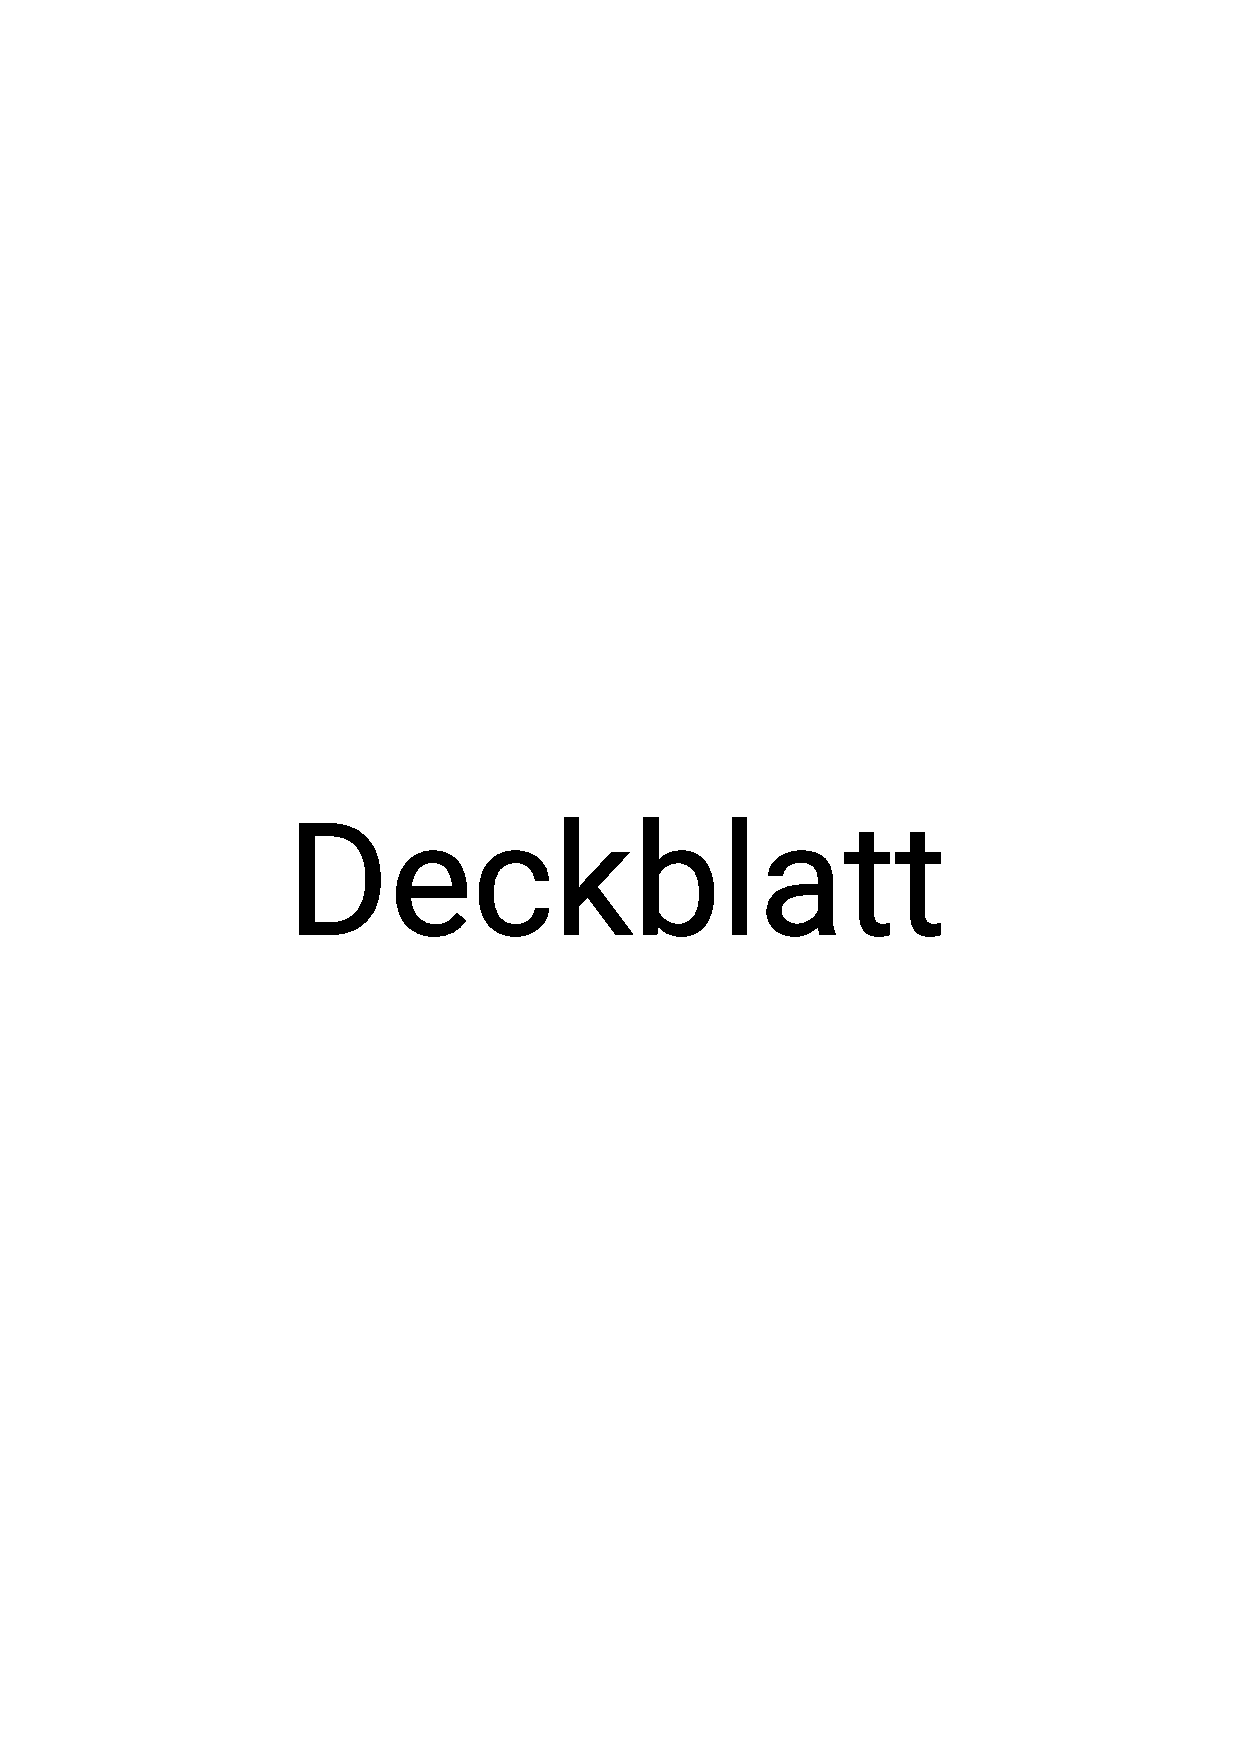
\includepdf{deckblatt.pdf}

% \maketitle
\begin{titlepage}
    \includepdf{titelblatt/titelblatt.pdf}
\end{titlepage}

%\frontmatter

% An dieser Stelle kann die Gendererklärung erzeugt werden, sofern sie notwendig
% sein sollte. Um eine zu erzeugen, einfach das Prozentzeichen entfernen.
% \gendererklaerung

\chapter*{Abstract}\label{chapter:Abstract}
%\addcontentsline{toc}{chapter}{Abstract} (Soll in Dachsberg nicht im Inhaltsverzeichnis aufscheinen)
%
% _abstract.tex
% Dieses Dokument fällt nicht unter die LPPL, unter der die vwa.cls steht!
% 

% Datei, in der das Abstract der VWA formuliert wird. Es empfiehlt sich, für jedes
% andere Kapitel eine neue Datei anzulegen, um Umstellungen in der VWA (im Haupt-
% dokument "vwa.tex" im Hauptordner des Projekts) zu erleichtern.
% Abstract im Umfang von ca. 1000--1500 Zeichen

\thispagestyle{empty} %Nötig zum Unterbinden der Seitennummer (wird erst ab dem Inhaltsverzeichnis angezeigt)


\chapter*{Vorwort}\label{chapter:Vorwort}
%\addcontentsline{toc}{chapter}{Vorwort} (Soll in Dachsberg nicht im Inhaltsverzeichnis aufscheinen)
\thispagestyle{empty} %Nötig zum Unterbinden der Seitennummer (wird erst ab dem Inhaltsverzeichnis angezeigt)



% Hauptinhalt des Dokuments deklarieren
\mainmatter

% Inhaltsverzeichnis an dieser Stelle erzeugen
\setcounter{page}{4} %Die erste nummerierte Seite soll das Inhaltsverzeichnis (tableofcontents) sein.
\zeilenabstand{1.25}
\tableofcontents
\zeilenabstand{1.5}

\setcounter{figure}{0}
\counterwithout{figure}{chapter}

% Kapitel hier einbinden, bspw:
% 1_einleitung.tex
% Beispieldatei mitgeliefert mit der vwa.cls von Alexander Leithner
% Dieses Dokument fällt nicht unter die LPPL, unter der die vwa.cls steht!
% 

% Datei, die das Schreiben von Kapiteln für die VWA in LaTeX demonstrieren
% soll. Alle Kapitel müssen im Hauptdokument "vwa.tex" im Hauptordner des
% Projekts wie in Zeile 108 gezeigt, eingebunden werden!

\chapter{Einleitung}

\input{kapitel/kapitel_neuro_netze.tex}
\input{kapitel/kapitel_implementation_connect_four.tex}
\input{kapitel/kapitel_auswertung_ergebnisse.tex}
\input{kapitel/kapitel_schluss_und_aussicht.tex}
% (Prozentzeichen entfernen, um Befehl gültig zu machen)

% Anhang des Dokuments deklarieren (Dieser Befehl würde Glossar, Abbildungsverzeichnis etc. aus dem Inhaltsverzeichnis ausklammern)
%\appendix
% Anhang-Trennseite hier erzeugen: (nicht notwendig)
%\addpart*{Anhang}

%Literaturverzeichnis einbinden
% \chapter*{Literaturverzeichnis}\label{chapter:Literaturverzeichnis}
% \addcontentsline{toc}{chapter}{Literaturverzeichnis}
% %
% _literaturverzeichnis.tex
% Dieses Dokument ist für die händische Zitation in Dachsberg nötig
% 


% Literaturverzeichnis hier erzeugen (wird in Dachsberg nicht verwendet)
% \nocite{*}
\renewcommand{\bibname}{Literaturverzeichnis}
% \printbibliography
% \bibsection
\newpage
\bibliography{vwa}


% Abbildungsverzeichnis hier erzeugen: (wird in Dachsberg nicht verwendet)
% \addcontentsline{toc}{chapter}{\listfigurename}
% \listoffigures
% \linespread{-0.5}
% {
% \let\oldnumberline\numberline
% \renewcommand{\numberline}{\figurename:~\oldnumberline}
%     \listoffigures
% }

% Abbildungsverzeichnis einbinden  (falls nicht benötigt, bitte jede Zeile mittels % auskommentieren)
\chapter*{Abbildungsverzeichnis}\label{chapter:Abbildungsverzeichnis}
\addcontentsline{toc}{chapter}{Abbildungsverzeichnis}
%
% _abbildungsverzeichnis.tex
% Dieses Dokument ist für die (händische) Zitation der Abbildungen in Dachsberg nötig
% 

% Aufbau:
% 
% Abb. 1: Titel\dotfill 1\\\kurzzitat[.][]{quelle}


% Glossar einbinden (falls nicht benötigt, bitte jede Zeile mittels % auskommentieren)
% \chapter*{Glossar}\label{chapter:Glossar}
% \addcontentsline{toc}{chapter}{Glossar}
% %
% _glossar.tex
% Dieses Dokument muss nicht verpflichtend eingebunden werden.
% 



% Anhang einbinden  (falls nicht benötigt, bitte jede Zeile mittels % auskommentieren)
\chapter*{Python Umgebung und Libraries}\label{chapter:Python Umgebung und Libraries}
\addcontentsline{toc}{chapter}{Python Umgebung und Libraries}
%
% _anhang.tex
% Dieses Dokument muss nicht verpflichtend eingebunden werden.
% 


% Selbstständigkeitserklärung hier erzeugen: (in Dachsberg separat)
% \selbststaendigkeitserklaerung

% Dokumentenende markieren, es darf kein Inhalt folgen!
\bibliographystyle{dachsberg}
\end{document}
